% Created:  Sun 15 Jun 2014 04:25 pm
% Author:   Josh Wainwright
% Filename: introduction.tex
\part{Introduction}
\label{prt:introduction}

\section{Medical Imaging}
\label{sec:section_name}

% TODO reword first sentence.
In various scientific fields, viewing and imaging objects smaller than the
human eye can naturally observe, is an ability eagerly sought. Microscopy in
medical fields has allowed us to learn about the nature of tissues,
micro-organisms and cells and the way they work together and to develop
preventative measures and cures for injuries and diseases.

The humble microscope, used as far back as the 1500's, is able to show us a
world that is not usually visible. In recent times, as our understanding has
grown, we have desired to see beyond what ordinary microscopes are capable of
and have invented machines that let us catch a glimpse of some of the smallest
structures in biology---molecules. However, when the objects to be viewed get
this small, of the order of a few tens of nanometers, the light that is used to
view them becomes the limiting factor.

% \section[Sub-Diffraction-Limit Imaging]{Sub-Diffraction-Limit\\ Imaging}
\section{Sub-Diffraction-Limit Imaging}
\label{sec:sub_diffraction_limit_imaging}

Imaging objects becomes more difficult as they get smaller because of the
wavelength of light ($\lambda$). Once two objects are separated by a distance
of an order similar to that of the wavelength of the light used to view them,
it is no longer possible to resolve these two objects apart. Instead all that
can be seen is a blur of the two objects together.

There have been several techniques developed for distinguishing objects apart
on smaller and smaller scales. Many of these involve using different
wavelengths of light.  For example, instead of being limited by visible light,
$\lambda \approx 5\times 10^{-7} \textrm{m}$, x-ray radiation ($\lambda \approx
10^{-10} \textrm{m}$) or even electrons ($\lambda \approx 10^{-11} \textrm{m}$)
can be used to resolve smaller scales in x-ray and electron microscopy
respectively. The smaller wavelengths imply higher energies however, meaning
that there is the danger of destroying the sample.

The minimum separation at which two objects can be resolved is given by Abbe's
criterion, $d$,

\begin{align}
	d &= \frac{\lambda}{2N\!A} \\
	  &= \frac{\lambda}{2n\sin\theta},
\end{align}

where $N\!A$ is the numerical aperture of the microscope, the range of angles
that the microscope's lens will let light through properly, $n$ is the
refractive index of the lens material and $\theta$ is the angle at which the
light is incident on the lens. For typical values of $\lambda \approx
\SI{500}{\nano\metre}$ (in the middle of the visible range), and $N\!A = 1.5$,
the maximum resolving distance is $d = \SI{160}{\nano\meter}$, this is the
diffraction limit. This is an order of magnitude larger than the objects that
need to be resolved. A few attempts to avoid this limit using exotic types of
lenses have been developed\cite{fang2005sub}, but these are currently far more
expensive to use than traditional imaging equipment.

\subsection{Image Manipulation}
\label{sub:image_manipulation}

Instead of trying to avoid the diffraction limit using shorter wavelengths of
light or particles, other techniques employ different methods of actually
capturing the image, and/or cleaver manipulation of the images that are
produced to get around the limitations of the diffraction problem.

For example Stochastic Optical Reconstruction Microscopy (STORM)
\cite{rust2006sub} and Photo-Activation Localisation Microscopy
(PALM)\cite{owen2010palm} use a technique where the objects to be imaged are
molecules of a fluorescent dye. These are attached to the object of interest, a
cell or sample of tissue for example. The type of dye molecule used allows the
fluorescence to be switched on and off, allowing some markers to be imaged
separately to others, effectively increasing the distance between points. Once
an image is captured, the point spread function (PSF) of the image of a marker
is used to locate the single point location of that marker, the ``on'' markers
are turned off and different ones turned on and the image retaken.  When many
of these images are taken, they can be combined to provide accurate information
on the original location of the markers and hence the shape and dimensions of
the object.

\begin{figure}[tbh]
	\centering
	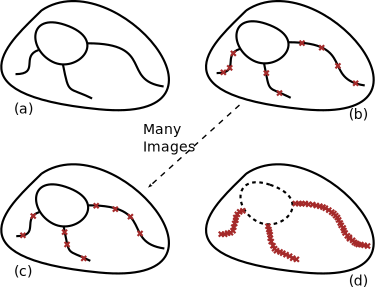
\includegraphics[width=7cm]{STORM.pdf}

	\caption[Creation of a STORM image.]{STORM imaging. (a) The actual
		structure to be imaged is too small for regular microscopy. In stages
		(b) through (c), many images are taken, each with a different subset of
		the fluorescent markers activated. When the images are combined, (d),
		the points add up and reveal the nature of the object.}\label{fig:STORM}
\end{figure}

The aim of this project is to provide a means by which the results of this
method of imaging can be analysed more efficiently and with a greater degree of
accuracy. This will take the form of a plugin for a piece of popular image
processing software called ImageJ.

The main deliverable is a plugin for extracting clusters of points from large
data sets for ImageJ. This plugin is written in Java and makes use of the
ImageJ Java API\cite{imagejapi}.

The sections included in this report are detailed below.

\begin{description}
	\item[\fullref{prt:introduction}] \hfill \\
		A brief background to the project with information about the type of
		data to be managed.

	\item[\fullref{prt:existing_cluster_analysis_algorithms}] \hfill \\
		A discussion of the existing algorithms that are in use for different
		applications and the reasons they do not fulfill the requirements of
		this project.

	\item[\fullref{prt:custom_algorithm}] \hfill \\
		A detailed examination of the algorithms that are developed in this
		project and the ways in which they are superior to the existing
		algorithms available.

	\item[\fullref{prt:imagej_plugin}] \hfill \\
		An explanation of the plugin that was developed for this project with
		information about how the constraints and variables of the algorithms
		are implemented in the plugin.

	\item[\fullref{prt:evaluation}] \hfill \\
		An evaluation of the success of the product at fulfilling the
		requirements given as well as of the processes and schedules that were
		followed during the project.

	\item[\fullref{prt:appendix}] \hfill \\
		A number of additional pieces of information and derivations to
		supplement the information in the body of this report.
\end{description}
